% !TeX program = xelatex
% Elsevier CAS single-column layout, following ICRL's CoFlexSim AES template.
\def\CoFlexUprightFonts{1}
\documentclass[a4paper,fleqn,longmktitle]{cas-sc}
\usepackage[numbers,sort&compress]{natbib}
\usepackage[nodots,compress]{numcompress}
\usepackage[mathlines]{lineno}
\usepackage{iftex}
\usepackage{newfloat}
\DeclareFloatingEnvironment[fileext=loa,name=Algorithm,placement=htbp]{algorithm}
\usepackage[indLines=true,noEnd=false]{algpseudocodex}
\tikzset{algpxIndentLine/.style={draw=black!55,solid,line width=0.3pt}}
\makeatletter
\newcommand{\solveralgorithmcaption}[2]{%
  \par\hrule height .8pt\vskip 3pt
  \noindent#1\enspace #2\par\vskip 3pt\hrule height .4pt\vskip 3pt}
\AtBeginEnvironment{algorithm}{\let\@makecaption\solveralgorithmcaption}
\makeatother
\usepackage{placeins}
% Uniform, upright manuscript styling, including template-generated labels.
\usepackage{fontspec}
\setmainfont{Times New Roman}[BoldFont={Times New Roman},ItalicFont={Times New Roman},BoldItalicFont={Times New Roman}]
\setsansfont{Arial}[BoldFont={Arial},ItalicFont={Arial},BoldItalicFont={Arial}]
\setmonofont{Consolas}[BoldFont={Consolas},ItalicFont={Consolas},BoldItalicFont={Consolas}]
\usepackage[math-style=upright]{unicode-math}
\setmathfont{STIXTwoMath-Regular.otf}
\renewcommand{\boldsymbol}[1]{\symup{#1}}
\renewcommand{\mathbf}[1]{\symup{#1}}
\renewcommand{\mathcal}[1]{\symsfup{#1}}
\renewcommand{\em}{\upshape\mdseries}
\renewcommand{\bfseries}{\mdseries}
\renewcommand{\itshape}{\upshape}

\ExplSyntaxOn
\cs_if_exist:NF \vbox_unpack_clear:N
  { \cs_new_eq:NN \vbox_unpack_clear:N \vbox_unpack_drop:N }
\box_new:N \l_aes_abstract_box
\dim_new:N \l_aes_keywords_height_dim
\AddToHook{env/Abstract/before}{
  \dim_set:Nn \l_aes_keywords_height_dim { \box_ht:N \g_stm_key_box + \box_dp:N \g_stm_key_box }
  \vbox_set:Nw \l_aes_abstract_box
}
\AddToHook{env/Abstract/after}{
  \vbox_set_end:
  \dim_set:Nn \l_aes_keywords_height_dim {
    \dim_max:nn { 0pt } { \l_aes_keywords_height_dim - \box_ht:N \l_aes_abstract_box - \box_dp:N \l_aes_abstract_box } }
  \vbox_unpack_drop:N \l_aes_abstract_box
  \skip_vertical:n { \l_aes_keywords_height_dim }
}
\ExplSyntaxOff
\newcommand{\manuscripttitle}{Residual-Aware CAD Contact for Rigid Mechanisms with Certified Clearance Events}
\hypersetup{pdftitle={\manuscripttitle}}
\providecommand{\doi}[1]{\href{https://doi.org/#1}{\nolinkurl{#1}}}
\renewcommand\linenumberfont{\normalfont\tiny\sffamily\color{gray}}
\graphicspath{{figures/}}
\newcommand{\micron}{µm}
\newcommand{\microsec}{µs}
\newcommand{\norminf}[1]{\left\lVert #1\right\rVert_{\infty}}
\newcommand{\resultfigure}[3]{%
  \begin{figure}[pos=!htbp]\centering
  \includegraphics[width=.91\linewidth]{#1-model.png}\par\medskip
  \includegraphics[width=.91\linewidth]{#1-response.pdf}
  \caption{#2}\label{#3}\end{figure}}

\begin{document}
\title[mode=title]{\manuscripttitle}
\shorttitle{Residual-aware CAD contact}
\shortauthors{Manuscript for review}
% Add the confirmed author list, affiliations and correspondence before submission.
\begin{abstract}
Rigid mechanisms with small clearances require geometric queries that resolve the operating gap and supply sufficiently accurate loads for time integration. We present a CAD contact software framework that selects the accuracy of a contact-force evaluation from the nonlinear residual of an implicit time step. Force intervals bound the effect of geometric uncertainty on Newton convergence and line search. A relative displacement bound revalidates cached exclusions, and a separate clearance query uses the earliest surviving space--time region to construct feasible witnesses on the trimmed CAD boundary. Across 34 prescribed clearance paths, witness guidance increased the number resolved within the requested time width from 29 to 32. The three additional entries were resolved in 0.49--1.59 ms. Two closed-form impact models and three industrial mechanisms evaluate the dynamics. At a joint tolerance of 0.5~\micron{} in RMS displacement or transmission error and 2\% in RMS force, native CAD reduces time for the cam relative to the tested polygonal configurations and has comparable cost to a tuned polyline for the spur pair. The two-stage spur--helical reducer completed 90 input revolutions and admitted a 10~\microsec{} native step at the 1~\micron{}, 5\% tolerance. Bounded force evaluations certify the residual decisions and incur additional cost relative to direct force kernels.
\end{abstract}
\begin{keywords}
Rigid multibody dynamics \sep Boundary representation \sep Implicit time integration \sep Certified clearance \sep Contact geometry
\end{keywords}
\maketitle
\pagestyle{plain}
\thispagestyle{plain}
\linenumbers

\section{Introduction}
The clearance between moving components can be smaller than the geometric features that determine their contact. A pin can pass within micrometres of a trimmed rim, and a small shift of a tooth profile can change the temporal distribution of the mesh load. Tessellation allows established collision libraries to process such components, but resolving the remaining gap or the force waveform can require substantially finer geometry than a visual representation. The relevant engineering question is how much geometry and solver work a method needs at a prescribed response accuracy, and what information it can certify about the nominal CAD during motion.

Rigid contact simulation poses two different numerical decisions. In an implicit step, the solver asks whether the forces at a trial state satisfy the discrete equations and whether a further Newton trial improves them. In a clearance query, it asks whether every earlier pose stays above a specified separation and whether a feasible point pair establishes an entry. A force residual can tolerate a bounded local approximation. A certificate of clearance depends on an exclusion that holds over an entire interval of motion. We treat these two decisions through explicit numerical bounds on the CAD geometry and reuse information across nearby evaluations when those bounds permit it.

The contributions are as follows.
\begin{itemize}
\item We use force enclosures to control geometric evaluation in HHT integration. The residual interval decides whether a trial can be accepted or whether the geometry must be resolved more tightly. This gives the solver a force-accuracy criterion tied to its discrete equations.
\item We use the earliest surviving region of a continuous clearance search to construct feasible CAD witnesses. A verified witness tightens the upper end of a first-entry bracket while the interval search continues to establish the safe prefix. The strategy resolves near-threshold diagonal entries for which ordinary sampling exhausts the same work budget.
\item We revalidate earlier pair exclusions with a bound on relative point travel and use previously computed gear points to propose bounded ray intersections. We measure the cost of this reuse and distinguish it from the effect of using smooth CAD geometry in otherwise matched simulations.
\end{itemize}
We implement the methods in a C++ library with STEP import and evaluate them in three analytical fixtures, two single-stage mechanisms, and a two-stage reducer.

\section{Related work}
\paragraph{Contact on CAD boundaries.}
Crozet et al. compute multiple local minimum distances directly on smooth boundary representations and use them in rigid dynamics \citep{crozet2018}. Their analysis shows how continuous normals and geometry-specific culling can improve contact for rolling and sliding near small gaps. We build on this established use of smooth geometry. Our solver controls the uncertainty of the assembled generalized force and uses it to make nonlinear acceptance decisions. Our discrete comparison includes both general triangle-BVH queries and structure-aware polygonal queries with the same prescribed contact law.

\paragraph{Continuous collision and clearance.}
Geometric collision search between moving parametric surfaces can use derivative bounds to exclude regions of parameter space and time \citep{vonherzen1990}. Chen et al. construct time-dependent inclusion functions for time-linear parametric patches \citep{chen2024}. Their subsequent work analyses floating-point errors and benchmarks exact ground-truth collision times \citep{chen2026}. We consider positive clearance on trimmed STEP boundaries under a fixed-axis rigid motion and return separate lower and upper time bounds. The witness mechanism uses the search state to propose a point pair on a trimmed face and validates its distance before narrowing the time bracket. For triangular representations, inclusion-based CCD and rigid IPC accommodate, respectively, linearly moving primitive pairs with prescribed separation and curved rigid trajectories with barrier contact \citep{wang2021,ferguson2021}. Our numerical comparisons include a swept triangle BVH, static CAD-distance advancement, and a mesh-guided CAD check on the same prescribed paths.

\paragraph{Implicit integration and geometric accuracy.}
HHT introduces controllable numerical dissipation into time integration \citep{hht1977}. Inexact Newton methods allocate accuracy to the linear solve \citep{dembo1982}. Here the uncertain quantity is the contact force entering the nonlinear equations. Enclosing this force provides a conservative interval for the residual norm at each presented trial. Our time integration comparisons use native MuJoCo \citep{todorov2012}, Drake \citep{drakecontact}, and RecurDyn \citep{recurdyn} where their contact laws can be matched to the nominal experiment.

\section{Geometry and contact formulation}
\label{sec:geometry}
A component carries a nominal STEP boundary composed of parametric faces and trim curves. The importer extracts the finite face domains and prepares spatial bounds for the face patches and trim edges. The force query returns a generalized force estimate, an infinity-norm error bound, and a tangent for the nonlinear step. A prescribed-motion query bounds the onset of contact with an initial interval of inactivity and a feasible CAD point pair. Both queries use the nominal geometry and point-travel bounds, as shown in Fig.~\ref{fig:workflow}.

\begin{figure}[pos=!htbp]
\centering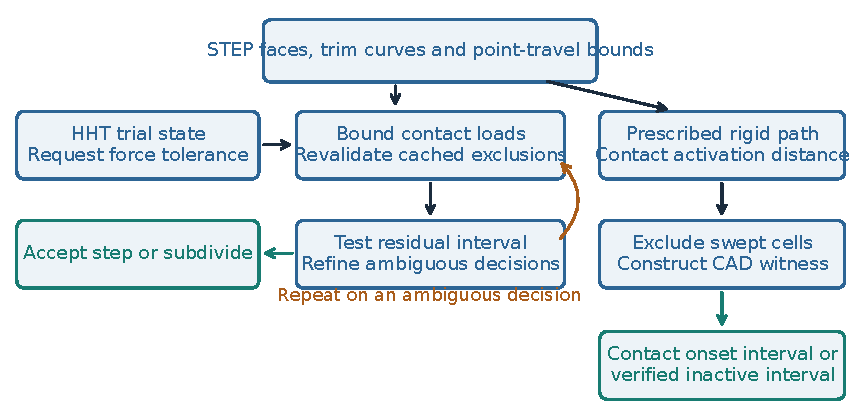
\includegraphics[width=.92\linewidth]{workflow.pdf}
\caption{Geometry queries on the original CAD boundary. The implicit solver controls the accuracy of the contact forces. The prescribed-motion query bounds contact onset.}
\label{fig:workflow}
\end{figure}

Let $Q$ denote the generalized configuration and $g_i(Q)$ the gap for contact pair or prescribed probe $i$. We use a frictionless normal force of the form
\begin{equation}
 \lambda_i(Q)=k_i [s_i-g_i(Q)]_+, \qquad
 F(Q,V,t)=F_{\mathrm{ext}}(Q,V,t)+\sum_i J_i(Q)^\top\lambda_i(Q),
 \label{eq:contact}
\end{equation}
where $s_i$ is the contact activation distance, $k_i$ is the stiffness, $J_i$ maps generalized velocities to relative normal motion, and $[b]_+=\max(0,b)$. The force activates as the pair moves into the contact layer $g_i<s_i$. Contact onset refers to the boundary of that layer. The primitive kernels use support points on spheres, cylindrical faces and finite planes. For a gear pair, the model prescribes candidate tooth pairs using the line of action. At each axial section, rays in the line-of-action direction intersect the two tooth profiles. The gap is the difference of ray coordinates multiplied by the cosine of the base helix angle. The axial quadrature and smooth shoulder weights at tooth entry and exit multiply the local stiffness. The angular lever arms follow the base radii projected by the same cosine. This model provides a normal force and an axial force component for each stage. Rigid axes carry the resulting projected torque, and the transmission stage has one shared shaft coordinate with its successor.

\subsection{Enclosing a gear section intersection}
\label{sec:gear-root}
The importer converts each sampled nonrational cubic flank section into B\'ezier spans. For a section $C(u)$, prescribed probe origin $p$, ray direction $n$ and transverse direction $w$, write $f(u)=w^\top(C(u)-p)$ and $h(u)=n^\top(C(u)-p)$. We seek the root of $f$ within the section and report $h$ there. Each B\'ezier control hull bounds the image of its span. If a global derivative bound is inconclusive, we exclude spans whose projected control hull misses the ray. We then bound $f'$ and $h'$ on the contiguous interval containing the surviving spans. Opposite signs at the ends and a one-sided $f'$ establish that the interval has a unique root $u^*$. For any $\hat u$ in the same interval the mean value theorem gives
\begin{equation}
 |h(u^*)-h(\hat u)| \leq \frac{\sup |h'|}{\inf |f'|}\, |f(\hat u)|.
 \label{eq:probe-error}
\end{equation}
We evaluate the right-hand side and the distance to the finite ray limits with outward-rounded intervals. A Newton root estimate supplies $\hat u$ when a previously evaluated point fails the current test. A span containing both the estimate and a sign change supplies tighter derivative bounds if needed. The stored point enclosure can propose a ray-coordinate interval at a new trial, where the root-existence, derivative and ray-limit checks apply again. We propagate the two accepted ray intervals through Eq.~\eqref{eq:contact}. A force-acceptable interval whose gap bound overlaps the sampled clearance floor is evaluated more tightly. The enclosures refer to the nominal extracted section polynomials. The gear model applies the local gap check at the sampled sections and trial states.

\section{Residual-controlled implicit integration}
\label{sec:method}
We use HHT-$\alpha$ for the reduced rigid coordinates, with $\alpha=-0.10$ in the reported runs. With a step size $\Delta t$, constant generalized mass $M$, and $a$ as the next acceleration, the predictors give $Q_{n+1}=Q_p+\beta\Delta t^2 a$ and $V_{n+1}=V_p+\gamma\Delta t a$, where $\beta=(1-\alpha)^2/4$ and $\gamma=1/2-\alpha$. The discrete force residual is
\begin{equation}
 R(a)=Ma-(1+\alpha)F(Q_{n+1},V_{n+1},t_{n+1})+\alpha F_n .
 \label{eq:residual}
\end{equation}
The force oracle accepts an absolute error budget $\eta_{\mathrm{req}}$ and returns $\widehat F$ and a bound $\eta$ on $\norminf{F-\widehat F}$. The accepted previous state retains its force bound $\eta_n$. The computed residual therefore differs from the nominal residual by at most
\begin{equation}
 \norminf{R-\widehat R} \leq |1+\alpha|\eta+|\alpha|\eta_n.
 \label{eq:resid-error}
\end{equation}
The implementation additionally encloses arithmetic in Eq.~\eqref{eq:residual} and bounds the norm componentwise in the numerical scaling of the generalized coordinates. If $[r^-,r^+]$ is the resulting interval for $\norminf R$, the trial converges whenever $r^+$ is at most the lower bound of the prescribed absolute-plus-relative tolerance. A trial with $r^-$ above the upper tolerance bound needs another Newton iteration. An overlap requests a tighter force estimate, as in Fig.~\ref{fig:residual}. A line search certifies descent only if the next residual upper bound is below the current lower bound. It refines the next interval, then the current interval if necessary, before re-evaluating that test. Algorithm~\ref{alg:trial} summarizes the solver.

\begin{figure}[pos=!htbp]
\centering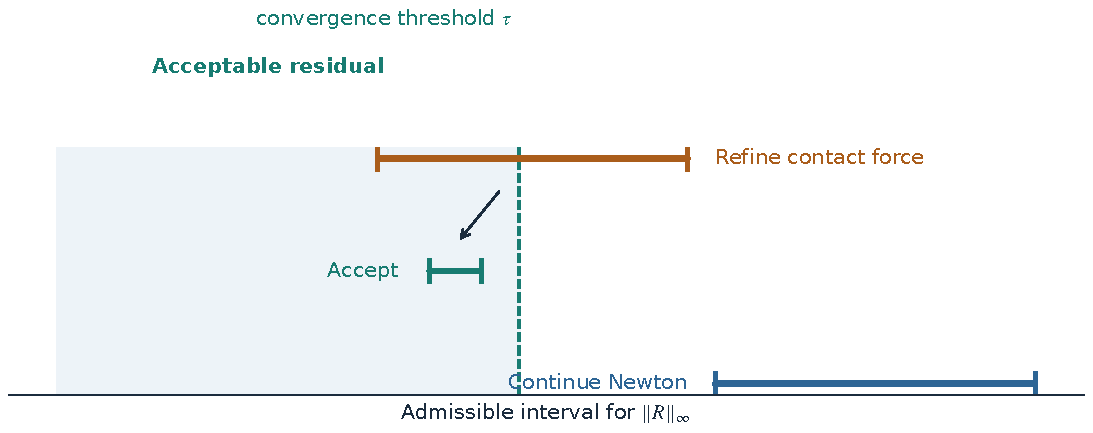
\includegraphics[width=.89\linewidth]{principle-residual.pdf}
\caption{Contact-force accuracy is sufficient when the residual interval decides the Newton test. An interval that overlaps the convergence threshold triggers a tighter force evaluation. During a line search the criterion tests the ordering of two residual intervals.}
\label{fig:residual}
\end{figure}

The first force budget scales with the prior force. Later budgets scale with the current residual, using the fraction $0.1$ after mapping through $1+\alpha$. Tight evaluation uses the finest available oracle. For primitive contact pairs, a lower gap bound $L_i>0$ and a bound $S_i$ on the normal Jacobian give the force contribution bound $k_i[s_i-L_i]_+S_i$. We sort unresolved contributions by this bound and may omit a tail when the sum of its bounds lies within the requested force budget. The actual force error includes the omitted sum and the interval widths of the evaluated contributions. The solver uses this actual error when the oracle exceeds the requested target. If the available precision cannot resolve an acceptance decision, the step may be subdivided within the prescribed limit.

\begin{algorithm}[!htbp]
\caption{HHT trial step with bounded contact evaluation}
\label{alg:trial}
\begin{algorithmic}[1]
\Require Prior state and force enclosure, time step $\Delta t$, residual tolerances
\State Form HHT predictors and set the trial acceleration from the prior state
\For{each allowed Newton iteration}
  \State Revalidate inactive-pair bounds at the trial configuration
  \State Evaluate contact loads using the requested budget and bound $\norminf R$
  \If{the residual interval overlaps the convergence tolerance}
     \State Request the finest available force evaluation and update the interval
  \EndIf
  \If{the upper residual bound satisfies the lower tolerance bound}
     \State \Return trial state and force bound if the applicable gap test also passes
  \EndIf
  \State Form the Newton direction from the current force tangent
  \State Check line-search trials and tighten overlapping residual intervals as needed
  \State Use the first trial with certified descent, or leave the iteration on failure
\EndFor
\State Subdivide the step if the subdivision budget remains
\end{algorithmic}
\end{algorithm}

\subsection{Reusing an exclusion}
A lower bound $L_0$ for the gap at configuration $Q_0$ remains useful at a nearby trial $Q$. For each body, let $d_A$ or $d_B$ bound the travel of every one of its material points between the two configurations. A translation contributes its magnitude and a rotation through $\Delta\theta$ about a fixed axis contributes at most $r |\Delta\theta|$, where $r$ bounds the distance of the surface from that axis. The triangle inequality holds for every point pair, so taking the infimum yields
\begin{equation}
 d(A(Q),B(Q)) \geq L_0-d_A-d_B.
 \label{eq:transport}
\end{equation}
If this lower bound exceeds $s_i$, the pair is inactive at $Q$. The cache stores its configuration and original lower bound. A trial outside the validity region in Fig.~\ref{fig:reuse} calls the ordinary gap query. A rejected trial cannot create a false exclusion because any stored state is rechecked according to Eq.~\eqref{eq:transport}. For linearly interpolated reduced coordinates on supported primitive pairs, each intermediate point is within half of the total step travel of one endpoint. The smaller endpoint lower bound minus half the total relative travel is therefore a conservative lower bound for the segment.

\begin{figure}[pos=!htbp]
\centering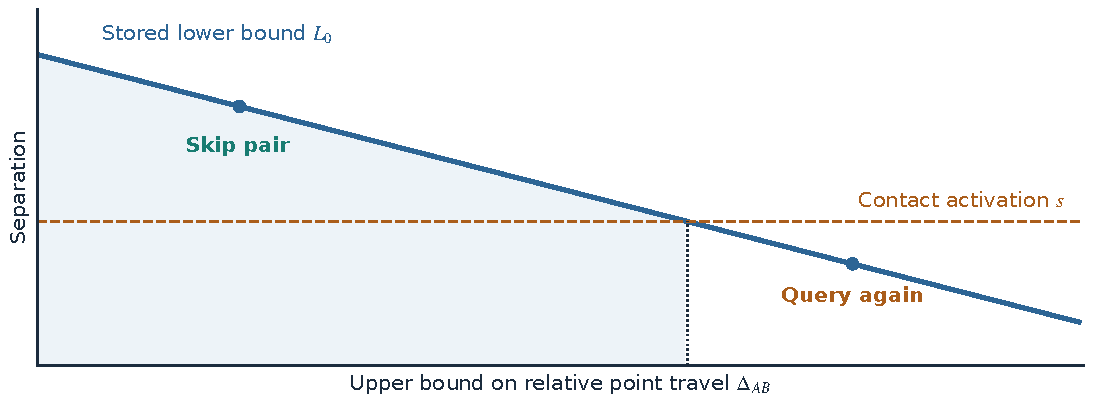
\includegraphics[width=.89\linewidth]{principle-reuse.pdf}
\caption{Validity of a stored separation bound at later Newton trials. The displacement bound can invalidate an exclusion as relative point travel grows.}
\label{fig:reuse}
\end{figure}

\section{Contact onset on a prescribed motion}
Consider a stationary boundary $A$ and a moving boundary $B(t)$ under a fixed-axis rotation with an affine translation. For a pair that starts outside the contact layer, the onset time is $t^*=\inf\{t:d(A,B(t))\leq s\}$, with $s$ the contact activation distance. The search combines enclosures of trimmed CAD cells with directional bounds on their relative motion. It excludes cells whose distance lower bound exceeds $s$ and processes the remaining cell-time windows in increasing order of start time. When the bounds are inconclusive the search splits cells or the time interval. A globally verified inactive interval ends at $t_-$. At any time $t_+$, a feasible CAD point pair whose outward distance upper bound is at most $s$ establishes $t^*\leq t_+$. The verification uses the point positions on the CAD, regardless of how they were proposed.

The interval search can advance the lower bound even when sampled points miss the region where contact begins. When a pair of trimmed cells survives the lower-bound tests, the general search evaluates feasible point pairs at the endpoints and midpoint of the surviving time window. The routine verifies both point parameters on the original boundary and tests their distance before updating $t_+$. At the work limit the search reports the verified inactive interval and any available upper time bound. Figure~\ref{fig:event-schematic} illustrates these results.

\begin{figure}[pos=!htbp]
\centering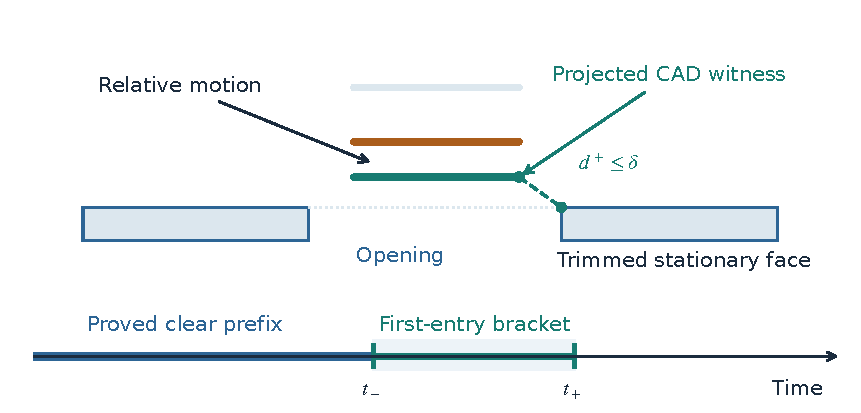
\includegraphics[width=.89\linewidth]{principle-event.pdf}
\caption{Bounding contact onset near a planar trim. A verified inactive interval ends at $t_-$, and the CAD point pair at $t_+$ satisfies the contact criterion.}
\label{fig:event-schematic}
\end{figure}

\subsection{Software interfaces}
The C++20 implementation separates geometry preparation, prescribed-motion search, and force evaluation. Prepared geometry is reused as poses and trajectory parameters change. The prescribed-motion query exposes the end of the verified inactive interval, an optional point pair with enclosing positions, and work counters. The force callback supplies force, stiffness, damping, and error information in the integrator's generalized coordinates. It also supports direct force evaluation for comparison. The verification tests check accepted residuals against a separate force evaluation, oracle behavior under a limit on attainable precision, and STEP import and query behavior.

\section{Numerical study}
\label{sec:evaluation}
The published reference cases test the timing of repeated contact transitions and the geometry of a cam with prescribed motion. The continuous detection study compares general geometry queries on complete STEP boundaries. Appendix~\ref{sec:industrial} reports the mechanism-specific force integration experiments.

The C++ implementations use Release builds and binary64 arithmetic. The Windows STEP runs use MSVC and Open CASCADE 7.9.3 on an AMD Ryzen 9 5900X. We give setup and online integration time separately and exclude trace serialization. Cam setup includes common model preparation. The fixed-step cam comparison uses three runs for each support query and one for each general search. The selected spur and reducer timings use three and two serial runs, respectively. We report the median online time for repeated configurations. The Linux engine results were obtained on the same workstation under WSL. The RecurDyn timings report the Windows solver and process interface separately. Software versions, individual timing records and precise settings are in the repository.

\subsection{Unilateral spring oscillator}
\label{sec:oscillator}
We reproduce the unit-mass oscillator of Junca and Rousselet \citep[Sec.~2]{junca2009}. Its displacement obeys $\ddot u+\omega_0^2 u+\varepsilon[u]_+=0$, with $u(0)=a_0>0$ and $\dot u(0)=0$. We use the normalizations $\omega_0=1$ and $a_0=1$ and select $\varepsilon/\omega_0^2=0.1$ for the parameterized model. The oscillator spends $\pi/\sqrt{\omega_0^2+\varepsilon}$ time units in contact and $\pi/\omega_0$ detached per period. Matching the two harmonic solutions at $u=0$ gives the displacement and contact force $\varepsilon[u]_+$ throughout the run.

We integrate 50 periods with the HHT solver and evaluate the scalar spring law directly. Linear interpolation of the numerical displacement at neighboring steps gives the times of contact onset and release. Each run reproduces all 100 transitions. Table~\ref{tab:oscillator} shows the refinement results. At the finest step, the largest timing error over the run is $2.09\times10^{-4}$ time units. The maximum errors in the duration of complete contact and detached intervals are $2.15\times10^{-6}$ and $2.05\times10^{-6}$ time units, respectively. Figure~\ref{fig:oscillator} shows the displacement and the accumulated timing error. This case tests integration through repeated changes of contact state with an exact force callback.

\begin{table}[pos=!htbp]
\centering\small
\caption{Errors over 50 periods of the published unilateral spring model. RMS displacement and force errors and the maximum onset or release timing error use the normalized units of the reproduction.}
\label{tab:oscillator}
\begin{tabular}{lrrr}\toprule
Nominal step & RMS displacement error & RMS force error & Max. timing error \\\midrule
0.0100 & $1.44\times10^{-3}$ & $1.01\times10^{-4}$ & $3.35\times10^{-3}$ \\
0.0050 & $3.60\times10^{-4}$ & $2.52\times10^{-5}$ & $8.37\times10^{-4}$ \\
0.0025 & $9.01\times10^{-5}$ & $6.29\times10^{-6}$ & $2.09\times10^{-4}$ \\
\bottomrule\end{tabular}
\end{table}

\begin{figure}[pos=!htbp]
\centering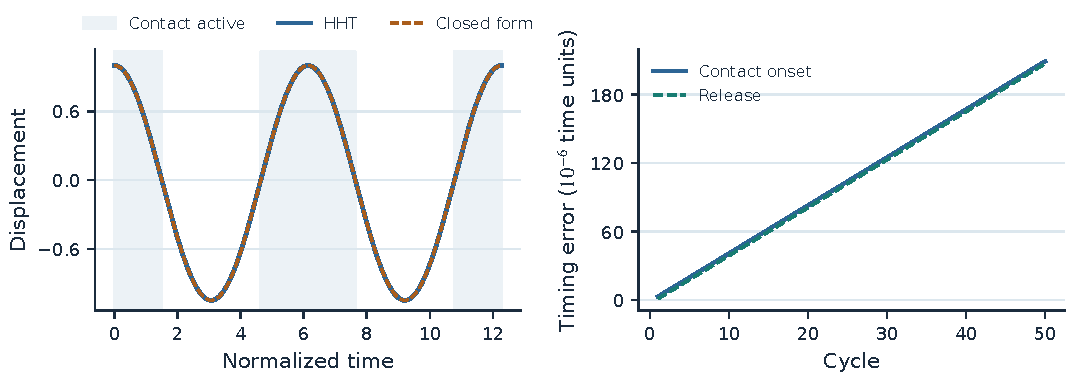
\includegraphics[width=.92\linewidth]{unilateral-response.pdf}
\caption{Unilateral oscillator with the finest HHT step. The first two periods show the motion and intervals of active contact. The onset and release timing errors are shown for all 50 periods.}
\label{fig:oscillator}
\end{figure}

\subsection{Constant-breadth cam and translating flat follower}
\label{sec:constant-breadth}
We reconstruct the Type I cam in Dhande and Rajaram's Example~1 \citep{dhande1984} from the six circular arcs of their Table~1. We use $a=6$, $b=5$, $c=7$, $d=2.5$, and $x_0=y_0=0$ in their length units. The cam rotates at $1$ rad/s between two parallel follower faces. Its constant breadth is $9$ length units. The guide and the opposing faces prescribe the follower translation. The reference comprises their displacement, velocity and acceleration equations over one complete revolution (Eqs.~(8), (10), and (12) and Table~2).

We rotate the reconstructed B-rep and obtain displacement from its supporting position along the follower translation axis. Position evaluation uses the CAD profile and its oriented extrema. Five-point finite differences at a spacing of $0.05^\circ$ yield velocity and acceleration. At the six arc junctions the acceleration changes discontinuously, so we report derivative errors at the 7,175 positions with stencils wholly inside an arc's contact interval. The maximum absolute CAD reconstruction errors are $2.66\times10^{-15}$ in displacement, $4.50\times10^{-12}$ in velocity and $1.31\times10^{-8}$ in acceleration, in the corresponding length and second units. Figure~\ref{fig:constant-breadth} shows the reconstructed motion and reference.

On the original $1^\circ$ sample grid we also import the CAD profile's extruded arc faces from STEP and use our bounded distance query to obtain a follower position interval at each pose. The 361 intervals, including both endpoints, contain the published position. The widest interval is $9.99\times10^{-5}$ length units and the maximum midpoint error is $4.91\times10^{-5}$ length units. This case verifies contact geometry and prescribed kinematics across all six profile sections.

\resultfigure{constant-breadth}{Reconstructed constant-breadth cam at $90^\circ$ between two translating flat faces, with an enlarged view of the contact on the right face. CAD kinematics and published solutions use the original length units and time in seconds. Acceleration curves are broken at the arc junctions.}{fig:constant-breadth}


\subsection{Continuous contact on complete CAD boundaries}
\label{sec:general-contact}
Our backend prepares each STEP boundary as trimmed patches and searches over the specified rigid motion. The tests use the same patch and trim operations for every shape. The axial-envelope shortcut and planar witness proposals are disabled. The mesh baselines use swept triangle prisms for translations and a triangle BVH distance query with a point-speed bound for rotation. We also test advancement with either bounded static B-rep distances or the independent numerical Open CASCADE distance kernel. For numerical distances the advancement uses a $10^{-6}$ mm margin. The numerical margin and mesh deflection do not give an outward enclosure of the nominal CAD surface.

\paragraph{Rotating cam with recorded contact transitions.}
We replay 22 accepted steps at contact onset from the eccentric-cam start-up and the immediately preceding step for each. Each replay keeps the recorded end poses and interpolates the angle and follower displacement within the step. The backends receive the two full STEP shapes and the rigid motion. The analytic cylinder--plane gap is evaluated separately at high precision to score the outcomes. The requested time width is $5\times10^{-4}$ of the 125~\microsec{} input step. The direct search and bounded static advancement each use a 20,000-task cap.

\begin{table}[pos=!htbp]
\small\centering
\caption{Rotating cam. An onset completes if its interval includes the reference time and meets the requested width. A preceding interval completes if it is reported inactive throughout. Query time is the median across all 44 paths after taking the median of two runs per path. It includes unresolved queries and excludes preparation.}
\label{tab:cam-onset}
\begin{tabular}{lrrr}\toprule
Method & Onsets (of 22) & Inactive (of 22) & Query (ms) \\\midrule
Direct B-rep interval search (ours) & 0 & 0 & 524.12 \\
Bounded B-rep distance + advancement & 0 & 0 & 300.76 \\
OCCT distance + advancement & 3 & 22 & 132.32 \\
Triangle BVH + advancement & 4 & 22 & 64.10 \\
\bottomrule\end{tabular}
\end{table}

Our search witnesses contact in three paths with brackets wider than the target and returns unresolved outcomes in the others. OCCT and the finest mesh report contact in all 22 onset paths. Most intervals are wider than the target. The mesh row uses a nominal deflection of 6.10 nm and requires 23.97 s of one-time mesh preparation. At 3.125~\micron{} deflection, 21 of the 22 onset paths disagree with the analytic reference. The data retain all six tessellation settings and the result of the mesh-guided CAD verification.

\paragraph{Production STEP assembly motions.}
We also run eight translation paths on the published OpenAMRobot MMP wheel and lidar assemblies and the Voron Trident Front Idler B assembly. All methods use the same original occurrences and path definitions. The requested bracket width is $5\times10^{-4}$ of the prescribed path duration, and B-rep search uses a 200,000-task cap. We compare the outputs with an adaptive numerical OCCT reference. This reference shares its distance kernel with the OCCT advancement baseline.

\begin{table}[pos=!htbp]
\small\centering
\caption{Production STEP translations. Completed results meet the requested width or exclude contact over the entire path and agree with the numerical reference. The reference remains unresolved on one of the eight paths. Online time is the median over all paths of three-run medians, excluding preparation.}
\label{tab:production-contact}
\begin{tabular}{lrr}\toprule
Method & Completed and compatible & Query (ms) \\\midrule
Direct B-rep interval search (ours) & 6 of 8 & 1034.05 \\
Bounded B-rep distance + advancement & 3 of 8 & 4609.70 \\
OCCT distance + advancement & 7 of 8 & 614.48 \\
Triangle BVH + swept-triangle CCD & 7 of 8 & 12.73 \\
Triangle CCD + bounded CAD advancement & 3 of 8 & 4814.83 \\
\bottomrule\end{tabular}
\end{table}

The mesh rows use the 3.125~\micron{} nominal deflection. The direct search completes the three wheel paths, the lidar pre-seat path and two idler paths. It retains a wider interval for full lidar insertion. The Voron spacer reference is unresolved, so that path contributes to the timing but has no success credit. The finest mesh and numerical OCCT methods agree with the reference on all seven resolved reference paths.


\paragraph{Loaded spur and reducer stages.}
We replay one 20~\microsec{} segment during the load rise for the spur pair and each reducer stage. Relative translation is interpolated between the recorded end poses in the driver frame. The deviations of these chords from the rotating center paths are bounded by 0.163~\micron{} under linear angular interpolation. The STEP boundaries are complete gear solids. Our search, OCCT advancement, and the finest tested triangle BVH report contact at the initial pose on all three segments. These checks exercise the same pipeline on involute and helical tooth surfaces under load. Each segment starts inside the contact layer, so this experiment has no onset time to localize within the step.

\paragraph{Chen et al.'s published patch example.}
We also run the official TDIB-CCD OBB solver \citep{chen2024} on its distributed \texttt{singleTest} case. Two orthogonal bicubic patches translate at the prescribed speeds. Their analytic intersection time is $10/17$ in the example's time units. The official implementation gives a candidate time of $0.5882353$ and a distance of $8.97\times10^{-4}$ between the returned parameter-cell centers. The median query time over five runs is 285.72 ms. The direct B-rep search proves the inactive interval up to $0.5882353$ and leaves the zero-distance witness unresolved at 25,000 tasks, with a median of 2,612.94 ms. This shared problem uses untrimmed patches and linear control-point motion. Matching the solver to the full STEP cases also requires trim-domain handling and an agreed model of rotating motion and contact activation.
\FloatBarrier



\section{Discussion}
Three factors account for the measured cost. First, for geometry that the mechanism revisits at every step, smooth support points and CAD flank roots avoid the resolution-dependent cost of a general triangle search. The specialized polygonal baselines remove most of that search cost and narrow the gap in runtime. Second, continuous clearance near a trim depends on obtaining both a lower time bound and a feasible witness. The guided query helps when the lower bound is already informative and ordinary samples miss the relevant rim region. Third, a bounded residual decision adds interval work to each contact evaluation. On these mechanisms the unbounded fixed CAD path is faster than the bounded variants. The speed of the native path and the numerical guarantees of the bounded path are distinct outcomes.

The residual test applies to force oracles that can enclose their own error. The implementations here cover frictionless compliance with positively separated surfaces, the primitive pairs in the validation cases, and projected sections of the tested nonrational cubic gear flanks. The full STEP clearance query accepts trimmed patches and the prescribed fixed-axis relative trajectories. Witness guidance currently accelerates planar-face proposals. At exact grazing the available finite work can yield a safe prefix and leave the event unresolved. The gear results establish feasibility for rotational transmission dynamics under the specified contact and axial quadrature. They use a sampled projected gap for gear trials. The continuous clearance certificate applies to the prescribed query paths and to the guarded primitive simulations within their supported path representation. Force-residual bounds control solution of the discretized equations. The trajectory errors also depend on the time step, contact law, and spatial quadrature.

\section{Conclusion}
The framework brings three numerical decisions into rigid CAD contact software. It asks how tightly a contact load must be resolved for an implicit step, whether an earlier separation exclusion still holds after a change of state, and whether a feasible CAD witness can close a clearance-event bracket. Guidance resolved three additional near-threshold trajectories, while the bounded HHT mode verified the force residual in the analytical cases and the supported mechanism runs. The industrial comparisons show that the cost advantage depends on the response tolerance and the geometric query available to the competing representation. Full force enclosures add cost to the direct CAD path. Their overhead identifies where cheaper enclosures and more selective refinement can improve the implementation.

\section*{Software and data availability}
The implementation, benchmark configurations, STEP model generators, measured summaries, and figure scripts are available in the accompanying \href{https://github.com/W-Moorer/NurbsCONTACT}{NurbsCONTACT repository}. The study protocol in the repository specifies the execution and reference settings. The RecurDyn runs require a licensed RecurDyn 2023 installation and its ProcessNet interface.

\bibliographystyle{model3-num-names}
\bibliography{references}
\end{document}
